%%%%%%%%%%%%%%%%%%%%%%%%%%%%%%%%%%%%%%%%%%%%%%%%%%%%%%%%%%%%%
\documentclass[11pt]{scrartcl} 
%########################### Preferences #################################

\usepackage{vmargin}
\usepackage{color}
\usepackage{amsthm}
\usepackage{amssymb}
\usepackage{amsmath}
\usepackage{amsfonts}
\usepackage{amstext}
\usepackage{amsbsy}
%\usepackage{mathbbol}
\usepackage{graphicx} 
\usepackage{verbatim}
\usepackage{csvsimple} 
\usepackage{subcaption}
%\usepackage{hyperref}
\usepackage{fancyhdr}
\usepackage{multirow}
\usepackage{listings}
\usepackage[numbers,sort&compress]{natbib}[2010/09/13]
\usepackage{mathptmx}

%  new definitions
\renewcommand{\div}{\bs{\nabla}\! \cdot \!}
\newcommand{\grad}{\bs{\nabla}}
\newcommand{\norm}[1]{\left\lVert#1\right\rVert_{L^2}}
% extra space
\newcommand{\qq}{\quad\quad}
% common reference commands
\newcommand{\eqt}[1]{Equation~\ref{#1}}                     % equation
\newcommand{\fig}[1]{Figure~\ref{#1}}                      % figure
\newcommand{\tbl}[1]{Table~\ref{#1}}                     % table
\newcommand{\sct}[1]{Section~\ref{#1}}                   % section
\newcommand{\app}[1]{Appendix~\ref{#1}}                   % appendix

\newcommand{\bs}[1]{\mathbf{#1}}
\newcommand{\dd}{\mathrm{d}}
\newcommand{\keff}{k_\textit{eff}}

\newcommand{\be}{\begin{equation}}
\newcommand{\ee}{\end{equation}}
\newcommand{\vn}{\vec{n}}
\newcommand{\vel}{\vec{\mathrm{v}}}
\newcommand{\adj}{\Phi^\dagger_0}
\newcommand{\tcr}[1]{\textcolor{red}{#1}}
\newcommand{\tcb}[1]{\textcolor{blue}{#1}}
 

% ********* Caption Layout ************
%\usepackage{ccaption} % allows special formating of the captions
%\captionnamefont{\bf\footnotesize\sffamily} % defines the font of the caption name (e.g. Figure: or Table:)
%\captiontitlefont{\footnotesize\sffamily} % defines the font of the caption text (same as above, but not bold)
%\setlength{\abovecaptionskip}{0mm} %lowers the distance of captions to the figure
\setlength\parindent{0pt}
\setlength{\oddsidemargin}{1in}
\setlength{\evensidemargin}{1in}
\setlength{\textwidth}{6.5in}
% ********* Header and Footer **********
% This is something to play with forever. I use here the advanced settings of the KOMA script

\title{\vspace{-30mm}\normalfont MEEN 673 Project}
\subtitle{\normalfont Nonlinear Finite Element Implementation of Time Dependent Radiation Diffusion}
\author{\normalsize \textbf{Zachary M. Prince} \\
		\normalsize MEEN 673 \\
		\normalsize Dr. J. N. Reddy}

\pagestyle{fancy}
\fancyhf{}
\lhead{Prince - MEEN 673 Project}
\rfoot{Final}
\cfoot{\thepage}


%%%%%%%%%%%%%%%%%%%%%%%%%%%%%%%% boxes
\usepackage{color}
\definecolor{myblue}{rgb}{.8, .8, 1}
\usepackage{empheq}

\newlength\mytemplen
\newsavebox\mytempbox

\makeatletter
\newcommand\mybluebox{%
    \@ifnextchar[%]
       {\@mybluebox}%
       {\@mybluebox[0pt]}}

\def\@mybluebox[#1]{%
    \@ifnextchar[%]
       {\@@mybluebox[#1]}%
       {\@@mybluebox[#1][0pt]}}

\def\@@mybluebox[#1][#2]#3{
    \sbox\mytempbox{#3}%
    \mytemplen\ht\mytempbox
    \advance\mytemplen #1\relax
    \ht\mytempbox\mytemplen
    \mytemplen\dp\mytempbox
    \advance\mytemplen #2\relax
    \dp\mytempbox\mytemplen
    \colorbox{myblue}{\hspace{1em}\usebox{\mytempbox}\hspace{1em}}}

\makeatother

%################ End Preferences, Begin Document #####################


%%%%%%%%%%%%%%%%%%%%%%%%%%%%%%%%%%%%%%%%%%%%%%%%%%%%%%%%%%%%%%%%%%%%%%%%%%%%%
%%%%%%%%%%%%%%%%%%%%%%%%%%%%%%%%%%%%%%%%%%%%%%%%%%%%%%%%%%%%%%%%%%%%%%%%%%%%%
\begin{document}
%%%%%%%%%%%%%%%%%%%%%%%%%%%%%%%%%%%%%%%%%%%%%%%%%%%%%%%%%%%%%%%%%%%%%%%%%%%%%
%%%%%%%%%%%%%%%%%%%%%%%%%%%%%%%%%%%%%%%%%%%%%%%%%%%%%%%%%%%%%%%%%%%%%%%%%%%%%
\maketitle
\pagenumbering{arabic}


%%%%%%%%%%%%%%%%%%%%%%%%%%%%%%%%%%%%%%%%%%%%%%%%
%%%%%%%%%%%%%%%%%%%%%%%%%%%%%%%%%%%%%%%%%%%%%%%%
\section{\bf Introduction}
%%%%%%%%%%%%%%%%%%%%%%%%%%%%%%%%%%%%%%%%%%%%%%%%
%%%%%%%%%%%%%%%%%%%%%%%%%%%%%%%%%%%%%%%%%%%%%%%%

This purpose of this paper is to detail a project involving the finite element implementation of a nonlinear system of partial differential equations.  The project focuses on the evaluation of the time dependent radiation diffusion equation \cite{Mousseau_2000,Knoll_1999}.  The implementation involves defining the weak form of the equations, developing the finite element model, and detailing the nonlinear iteration process. \\

The time dependent radiation diffusion equations are defined in \eqref{eq:RTE}.  Where $E$ is the photon energy and $T$ is the material temperature.
\begin{subequations}
\be 
\frac{1}{c}\frac{\partial E}{\partial t} - \div D_r \grad E = \sigma_a\left(aT^4-E\right)
\ee
\be 
C_v \frac{\partial T}{\partial t} - \div D_t \grad T = -c\sigma_a\left(aT^4-E\right)
\ee
\label{eq:RTE}
\end{subequations}

$C_v$ is the material specific heat. $c$ is the speed of light (photon). $a$ is the Stephan-Boltzmann constant. $D_r$ is the radiation diffusion coefficient defined by \eqref{eq:Dr}.  $D_t$ is the material (plasma) conduction diffusion coefficient defined by \eqref{eq:Dt}. Finally, $\sigma_a$ is the photon absorption cross-section defined by \eqref{eq:sa}.
\be
D_r(T) = \frac{1}{3\sigma_a}
\label{eq:Dr}
\ee
\be
D_t(T) = kT^{5/2}
\label{eq:Dt}
\ee
\be
\sigma_a(T) = \frac{z^3}{T^3}
\label{eq:sa}
\ee
Where $k$ is a constant and $z$ is the atomic mass number of the material. 


%%%%%%%%%%%%%%%%%%%%%%%%%%%%%%%%%%%%%%%%%%%%%%%%
%%%%%%%%%%%%%%%%%%%%%%%%%%%%%%%%%%%%%%%%%%%%%%%%
\section{\bf Finite Element Development}
%%%%%%%%%%%%%%%%%%%%%%%%%%%%%%%%%%%%%%%%%%%%%%%%
%%%%%%%%%%%%%%%%%%%%%%%%%%%%%%%%%%%%%%%%%%%%%%%%

%%%%%%%%%%%%%%%%%%%%%%%%%%%%%%%%%%%%%%%%%%%%%%%%
\subsection{\bf Weak Form}
%%%%%%%%%%%%%%%%%%%%%%%%%%%%%%%%%%%%%%%%%%%%%%%%

To develop the weak form, \eqref{eq:RTE} is multiplied by test functions ($u$ for the $E$ equation and $v$ for the $T$ equation) and integrated over elements.  The result is shown in \eqref{eq:weak}.

\begin{subequations}
\be 
\int_{\Omega^e}\left\lbrace \frac{1}{c}\frac{\partial E}{\partial t}u + \grad u \cdot D_r \grad E - \sigma_a\left(aT^4-E\right)u \right\rbrace + q_E = 0
\ee
\be 
\int_{\Omega^e}\left\lbrace C_v\frac{\partial T}{\partial t}v + \grad v \cdot D_t \grad T + c\sigma_a\left(aT^4-E\right)v \right\rbrace + q_T = 0
\ee
\label{eq:weak}
\end{subequations}
Where $q_E$ and $q_T$ are boundary contributions dependent on the boundary conditions.


%%%%%%%%%%%%%%%%%%%%%%%%%%%%%%%%%%%%%%%%%%%%%%%%
\subsection{\bf Finite Element Model}
%%%%%%%%%%%%%%%%%%%%%%%%%%%%%%%%%%%%%%%%%%%%%%%%

To develop the finite element model, the solutions and test functions are expanded in nodal values and shape function show in \eqref{eq:approx}.  These expansions are applied to \eqref{eq:weak} and shown in \eqref{eq:fem_tmp}
\be
E = \sum_{j=1}^N\psi_j E_j ; \qquad T = \sum_{j=1}^N\psi_j T_j; \qquad u = v = \psi_i 
\label{eq:approx}
\ee

\begin{subequations}

\be
\sum_{j=1}^N\int_{\Omega^e}\left\lbrace \frac{1}{c}\frac{\partial E_j}{\partial t}\psi_i\psi_j + \grad \psi_i \cdot D_r \grad \psi_j E_j - \sigma_a\left(aT^3T_j-E_j\right)\psi_i\psi_j \right\rbrace dxdy + q_E = 0
\ee

\be 
\sum_{j=1}^N\int_{\Omega^e}\left\lbrace C_v\frac{\partial T_j}{\partial t}\psi_i\psi_j + \grad \psi_i \cdot D_t \grad \psi_j T_j + c\sigma_a\left(aT^3T_j-E_j\right)\psi_i\psi_j \right\rbrace dxdy + q_T = 0
\ee

\label{eq:fem_tmp}
\end{subequations}

After applying material definitions from \eqref{eq:Dr}-\eqref{eq:sa}, \eqref{eq:fem_tmp} reduces to the form shown in \eqref{eq:fem}.

\begin{subequations}

\be
\sum_{j=1}^N\int_{\Omega^e}\left\lbrace \frac{1}{c}\frac{\partial E_j}{\partial t}\psi_i\psi_j + \grad \psi_i \cdot \frac{T^3}{3z^3} \grad \psi_j E_j - z^3\left(aT_j-\frac{E_j}{T^3}\right)\psi_i\psi_j \right\rbrace dxdy + q_E = 0
\ee

\be 
\sum_{j=1}^N\int_{\Omega^e}\left\lbrace C_v\frac{\partial T_j}{\partial t}\psi_i\psi_j + \grad \psi_i \cdot kT^{5/2} \grad \psi_j T_j + cz^3\left(aT_j-\frac{E_j}{T^3}\right)\psi_i\psi_j \right\rbrace dxdy + q_T = 0
\ee

\label{eq:fem}
\end{subequations}

The system can now be represented in matrix form shown in \eqref{eq:stiff} with matrix component definitions.

\begin{subequations}

\be
\begin{bmatrix} C^{11} & 0 \\ 0 & C^{22} \end{bmatrix}
\begin{bmatrix} \dot{E} \\ \dot{T} \end{bmatrix} +
\begin{bmatrix} K^{11} & K^{12} \\ K^{21} & K^{22} \end{bmatrix}
\begin{bmatrix} E \\ T \end{bmatrix} =
\begin{bmatrix} F^1 \\ F^2 \end{bmatrix}
\ee
\be 
C^{11}_{ij} = \int_{\Omega^e} \frac{1}{c} \psi_i\psi_j dxdy
\ee
\be 
C^{22}_{ij} = \int_{\Omega^e} C_v \psi_i\psi_j dxdy
\ee
\be 
K^{11}_{ij} = \int_{\Omega^e} \grad \psi_i \cdot \frac{T^3}{3z^3} \grad \psi_j dxdy + \int_{\Omega^e} \frac{z^3}{T^3}\psi_i\psi_j dxdy  + q_E(\psi_i,\psi_j)
\ee
\be 
K^{12}_{ij} = -\int_{\Omega^e} z^3a\psi_i\psi_j dxdy
\ee
\be 
K^{21}_{ij} = -\int_{\Omega^e} \frac{cz^3}{T^3}\psi_i\psi_j dxdy
\ee
\be 
K^{22}_{ij} = \int_{\Omega^e} \grad \psi_i \cdot kT^{5/2} \grad \psi_j dxdy + \int_{\Omega^e} cz^3a\psi_i\psi_j dxdy + q_T(\psi_i,\psi_j)
\ee
\be 
F^1_i = q_E(\psi_i)
\ee
\be 
F^2_i = q_T(\psi_i)
\ee

\label{eq:stiff}
\end{subequations}

%%%%%%%%%%%%%%%%%%%%%%%%%%%%%%%%%%%%%%%%%%%%%%%%
\subsection{\bf Time Discretization}
%%%%%%%%%%%%%%%%%%%%%%%%%%%%%%%%%%%%%%%%%%%%%%%%

The time discretization used for this project is defined by \eqref{eq:td}, where $U$ can be $E$ or $T$.
\be
\frac{U_{s+1}-U_s}{\Delta t} \approx \theta\frac{\partial U_{s+1}}{\partial t} + (1-\theta)\frac{\partial U_{s}}{\partial t}
\label{eq:td}
\ee

The finite element model can now be refactored into a new matrix form defined by \eqref{eq:fem_td} with coefficient definitions.  $U^1$ and $U^2$ correspond to $E$ and $T$, respectively.

\begin{subequations}

\be
\begin{bmatrix} \hat{K}^{11} & \hat{K}^{12} \\ \hat{K}^{21} & \hat{K}^{22} \end{bmatrix}
\begin{bmatrix} E \\ T \end{bmatrix}_{s+1} =
\begin{bmatrix} \hat{F}^1 \\ \hat{F}^2 \end{bmatrix}
\ee
\be 
\hat{K}^{\alpha\beta}_{ij} = \theta\Delta t K^{\alpha\beta}_{ij,s+1} + C^{\alpha\beta}_{ij} \qquad \alpha,\beta = 1,2
\ee
\be 
\hat{F}^{\alpha}_{i} = \sum_{\gamma=1}^2\sum_{j=1}^N\left[C^{\alpha\gamma}_{ij}-(1-\theta)\Delta tK^{\alpha\gamma}_{ij,s}\right]U^{\gamma}_{j,s} + \Delta t \left[\theta F^{\alpha}_{i,s+1}+(1-\theta)F^{\alpha}_{i,s}\right] \qquad \alpha=1,2
\ee

\label{eq:fem_td}
\end{subequations}

%%%%%%%%%%%%%%%%%%%%%%%%%%%%%%%%%%%%%%%%%%%%%%%%
\subsection{\bf Iteration Technique}
%%%%%%%%%%%%%%%%%%%%%%%%%%%%%%%%%%%%%%%%%%%%%%%%

Two types of iteration processes are necessary to analyze in this project. The first is direct or fixed-point iteration. Where the evaluation of the system described by \eqref{eq:fem_td} is iterated, updating $E$ and $T$ into $\hat{K}$, until convergence.  The second process is Newton iteration, where the tangent of the residual vector is evaluated.  A Newton iteration system can be described by \eqref{eq:tan_mat}. Where $T$ and $R$ correspond to the tangent matrix and residual vector, respectively.

\begin{subequations}

\be
\begin{bmatrix} T^{11} & T^{12} \\ T^{21} & T^{22} \end{bmatrix}
\delta \begin{bmatrix} E \\ T \end{bmatrix}_{s+1} =
-\begin{bmatrix} R^1 \\ R^2 \end{bmatrix}
\ee
\be 
R^{\alpha}_i = \sum_{\gamma=1}^2\sum_{j=1}^N\hat{K}^{\alpha\gamma}_{ij}U^{\gamma}_{j,s+1} - \hat{F}^{\alpha}_i \qquad \alpha=1,2
\ee
\be 
T^{\alpha\beta}_{ij} = \frac{\partial R^{\alpha}_i}{\partial U^{\beta}_{j,s+1}} \qquad \alpha,\beta = 1,2
\ee

\label{eq:tan_mat}
\end{subequations}

Applying the tangent matrix coefficient definition to \eqref{eq:stiff} results in the coefficients described in \eqref{eq:tan}.

\begin{subequations}

\be 
T^{11}_{ij} = \hat{K}^{11}_{ij}
\ee
\be 
T^{12}_{ij} = \hat{K}^{12}_{ij} + \theta\Delta t \left[ \int_{\Omega^e} \frac{T_{s+1}^2}{z^3} \left(\grad\psi_i\cdot\grad E_{s+1}\right)\psi_jdxdy - \int_{\Omega^e} \frac{3z^3}{T_{s+1}^4} E_{s+1} \psi_i\psi_jdxdy\right]
\ee
\be 
T^{21}_{ij} = \hat{K}^{21}_{ij}
\ee
\be 
T^{22}_{ij} = \hat{K}^{22}_{ij} + \theta\Delta t \left[ \int_{\Omega^e} \frac{5}{2}T_{s+1}^{3/2} \left(\grad\psi_i\cdot\grad T_{s+1}\right)\psi_jdxdy + \int_{\Omega^e} \frac{3cz^3}{T_{s+1}^4} E_{s+1} \psi_i\psi_jdxdy\right]
\ee

\label{eq:tan}
\end{subequations}

%%%%%%%%%%%%%%%%%%%%%%%%%%%%%%%%%%%%%%%%%%%%%%%%
%%%%%%%%%%%%%%%%%%%%%%%%%%%%%%%%%%%%%%%%%%%%%%%%
\section{\bf Examples}
%%%%%%%%%%%%%%%%%%%%%%%%%%%%%%%%%%%%%%%%%%%%%%%%
%%%%%%%%%%%%%%%%%%%%%%%%%%%%%%%%%%%%%%%%%%%%%%%%

%%%%%%%%%%%%%%%%%%%%%%%%%%%%%%%%%%%%%%%%%%%%%%%%
\subsection{\bf Quasi-1D Example}
%%%%%%%%%%%%%%%%%%%%%%%%%%%%%%%%%%%%%%%%%%%%%%%%

The first example comes from \cite{Mousseau_2000} which is a two-dimensional problem, but solution is constant in one direction.  The material properties, boundary and initial conditions are shown in \eqref{eq:init}. A 32X32, 64X64, 128X128, and 256X256 mesh was used with linear elements.  Reduced Newton-Cotes integration was used for all nonlinear terms, this insured that the temperature would be positive and not confuse the $D_t$ term. Backward Euler discretization ($\theta = 1$) was used with $\Delta t = 0.05$ and simulated 1.5 seconds.

\begin{subequations}
\be
z = c = a = C_v = 1.0 \qquad k = 0.1
\ee
\be 
E(x,y,0) = 1.0 \times 10^{-5} \qquad T(x,y,0) = (E(x,y,0)/a)^{1/4} = 5.62 \times 10^{-5}
\ee
\be 
\frac{1}{4}E-\frac{D_r}{2}\frac{\partial E}{\partial \vec{n}} = 1 \qquad x=0
\ee
\be 
\frac{1}{4}E+\frac{D_r}{2}\frac{\partial E}{\partial \vec{n}} = 0 \qquad x=1
\ee
\be 
\frac{\partial E}{\partial \vec{n}} = 0 \qquad y=0, x=0
\ee
\be 
\frac{\partial T}{\partial \vec{n}} = 0 \qquad \text{all boundaries}
\ee
\label{eq:init}
\end{subequations}

The results from \cite{Mousseau_2000} are shown in \fig{fig:ex1_paper} and the results of my simulations are in \fig{fig:ex1}.  It is important to note that the paper uses a different definition of $\sigma_a$ which, in practice, reduces the speed of the thermal wave by approximately half.  Therefore their transient lasted 3.0 seconds, but the shapes and magnitudes of the curves are comparable.

\begin{figure}[htpb!]
\centering
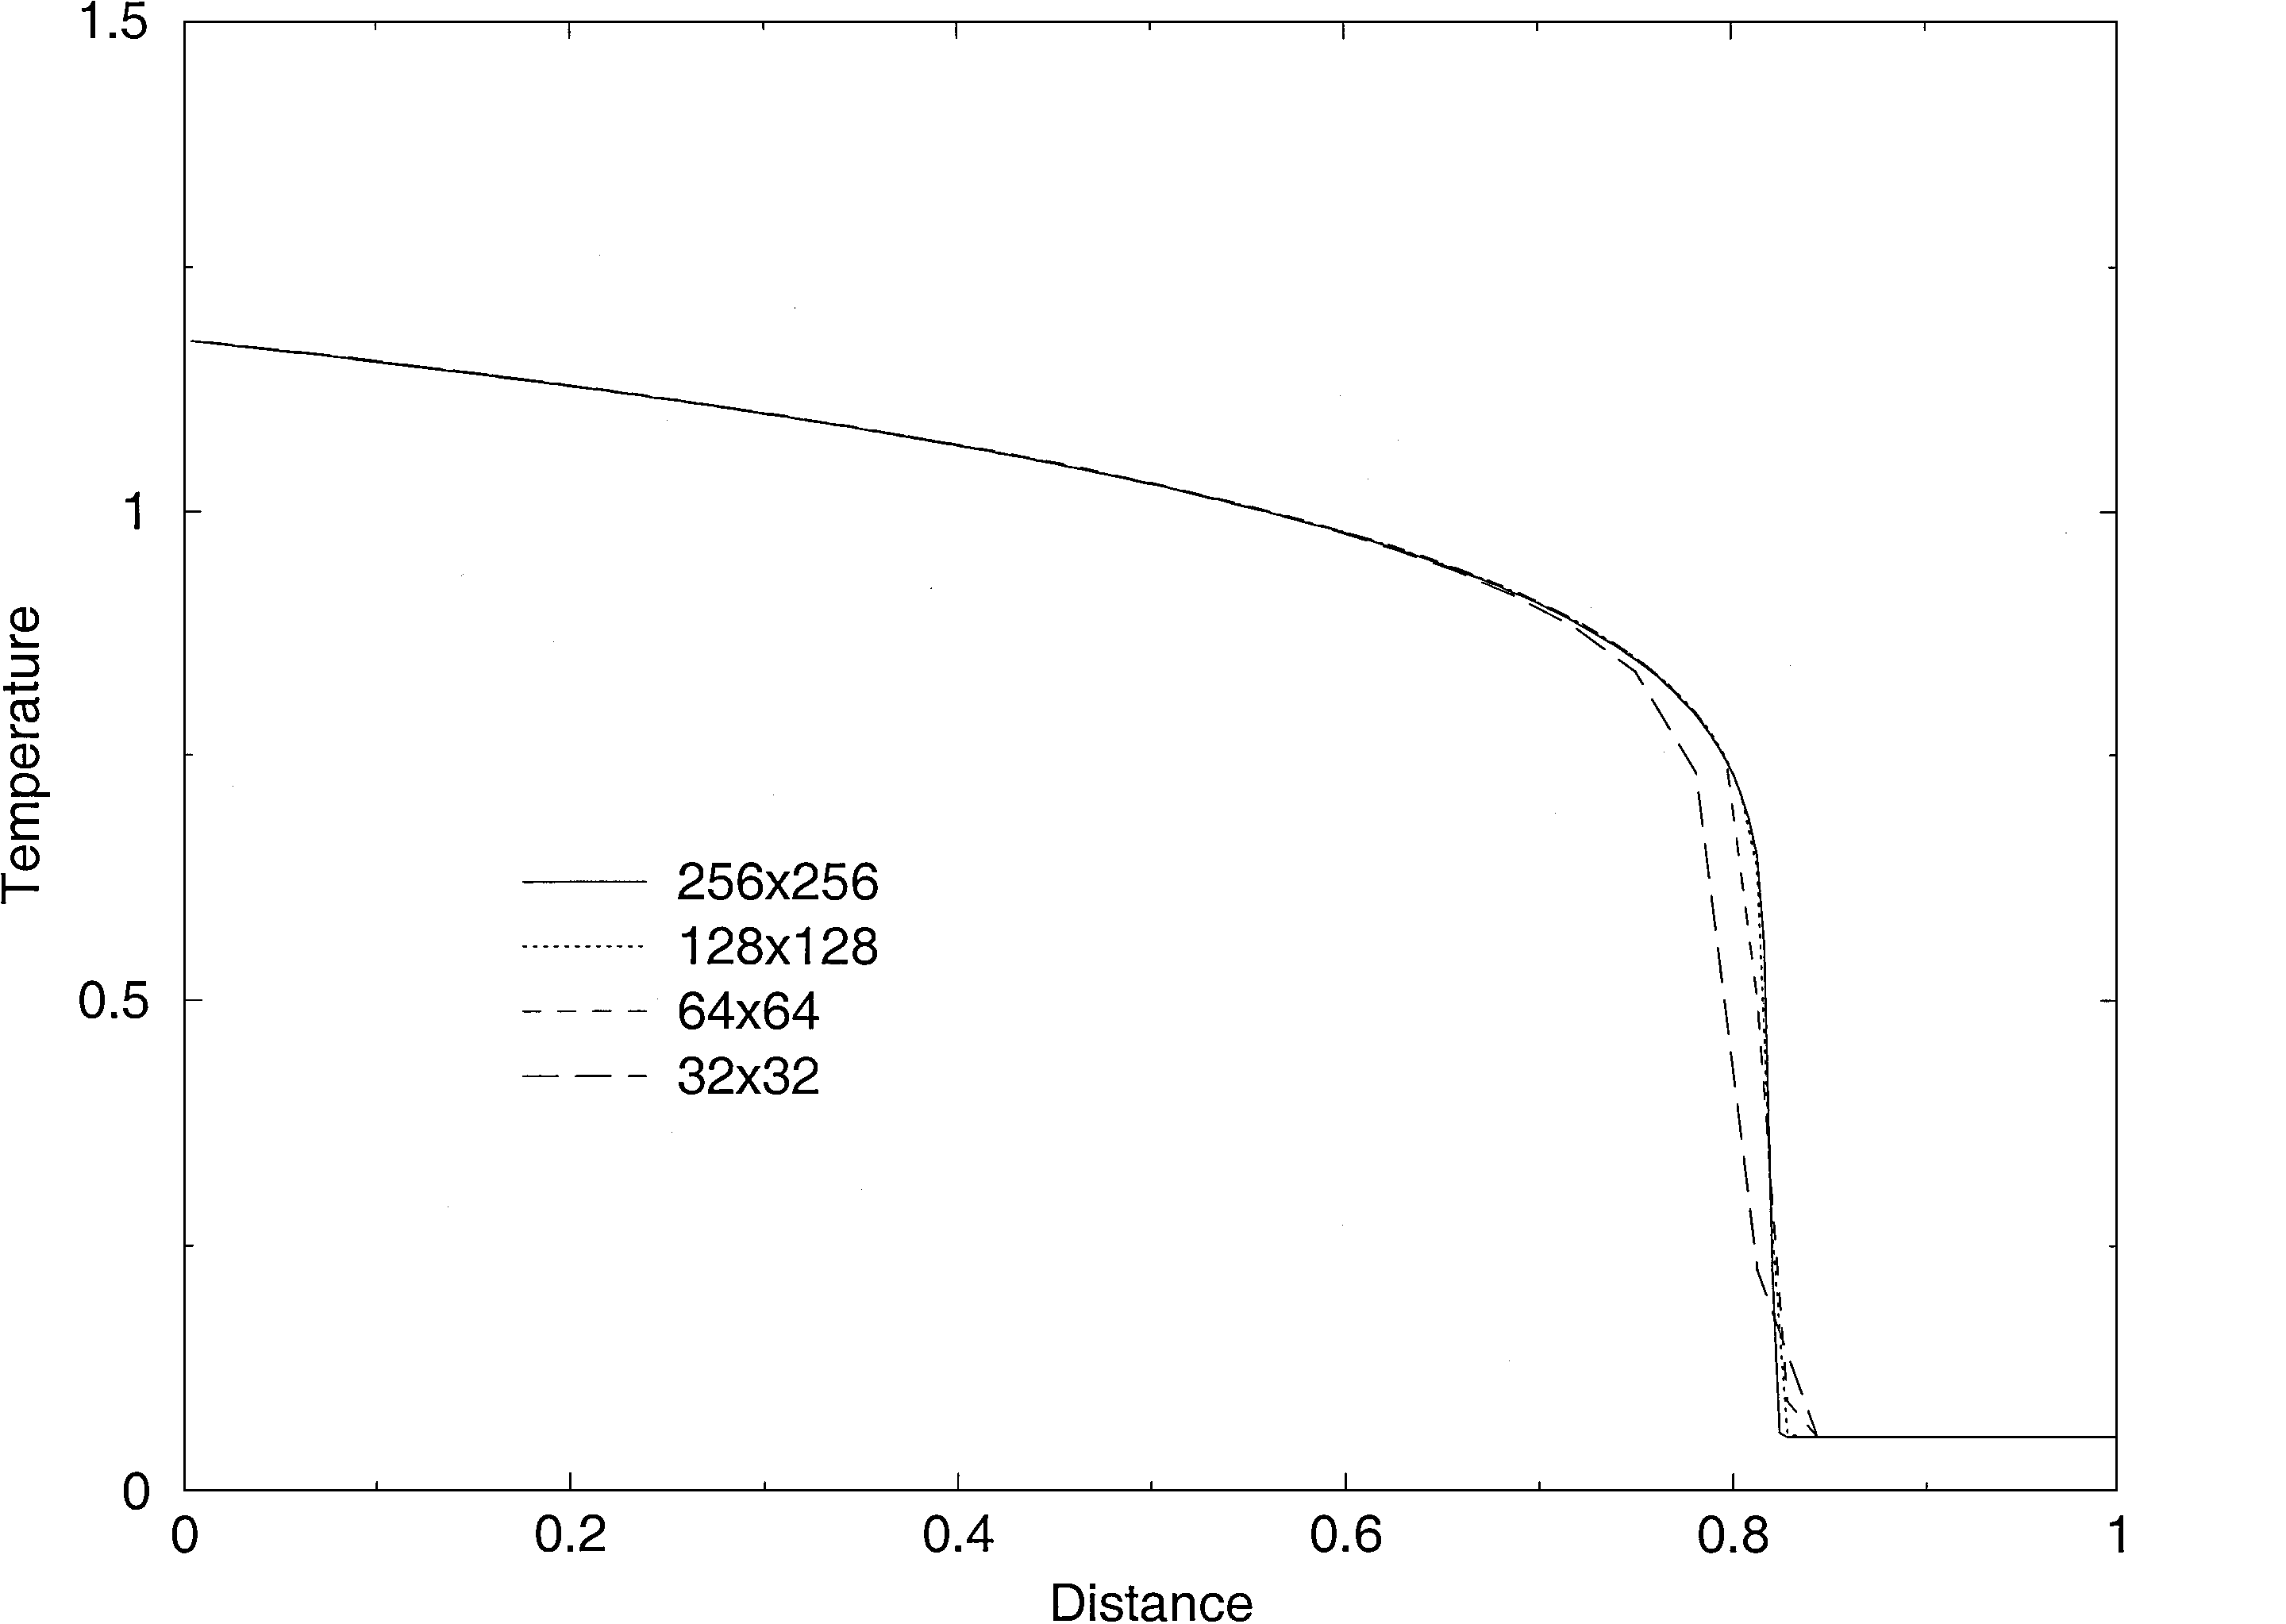
\includegraphics[width=0.75\linewidth]{Example1_paper.png}
\caption{Radiation temperature from \cite{Mousseau_2000}}
\label{fig:ex1_paper}
\end{figure}

\begin{figure}[htpb!]
\centering
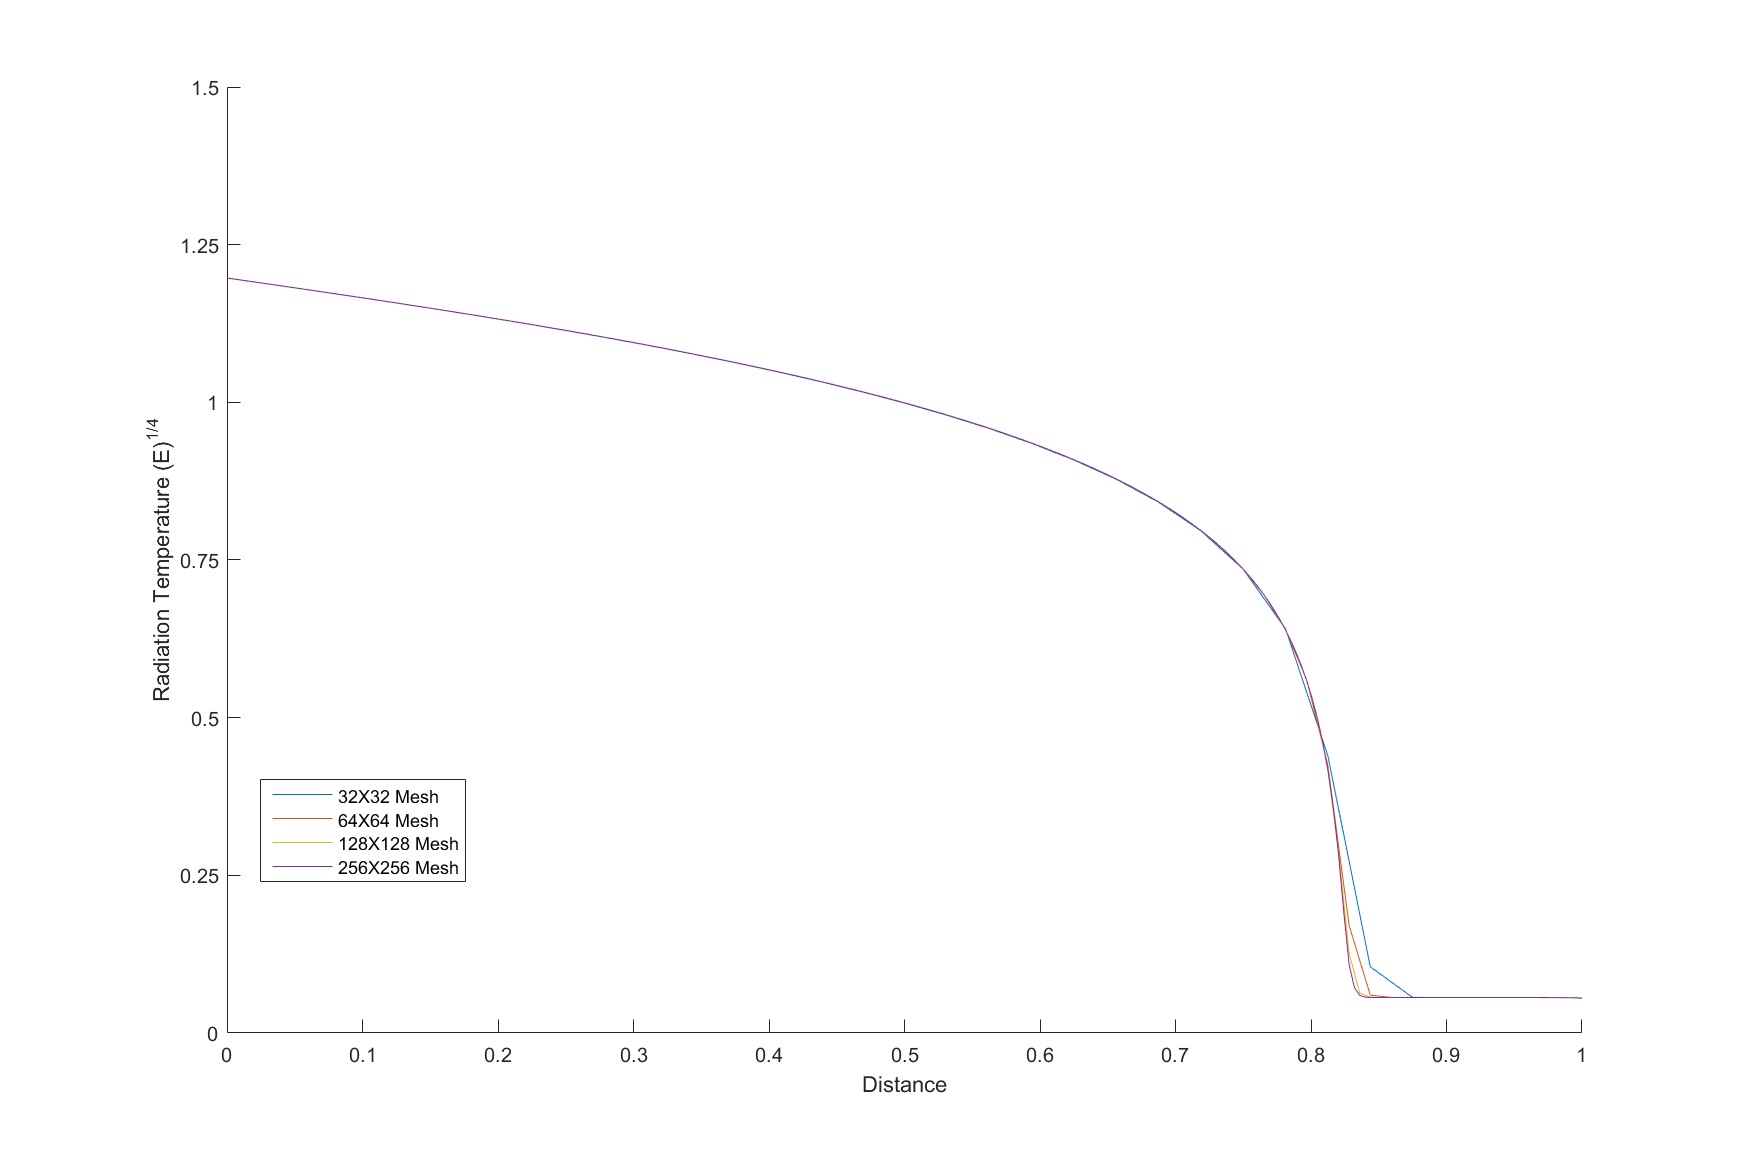
\includegraphics[width=\linewidth]{Example1.png}
\caption{Radiation temperature for Example 1}
\label{fig:ex1_paper}
\end{figure}

%%%%%%%%%%%%%%%%%%%%%%%%%%%%%%%%%%%%%%%%%%%%%%%%
\subsection{\bf Two Dimensional Example}
%%%%%%%%%%%%%%%%%%%%%%%%%%%%%%%%%%%%%%%%%%%%%%%%

This next example is exactly the same as the first to the first, except there is an opacity step in the middle of the domain.  This is implemented by varying $z$ in the domain, shown by \eqref{eq:z}.

\be 
z=\begin{cases}
Z \quad 1/3 \leq x,y \leq 2/3\\
1.0 \quad \text{otherwise}
\end{cases}
\label{eq:z}
\ee

Two cases were run: $Z=2.5$ and $Z=10.0$.  The material temperature for the cases are shown in \fig{fig:ex2_1} and \fig{fig:ex2_2} as contour plots, respectively.

\begin{figure}[htpb!]
\centering
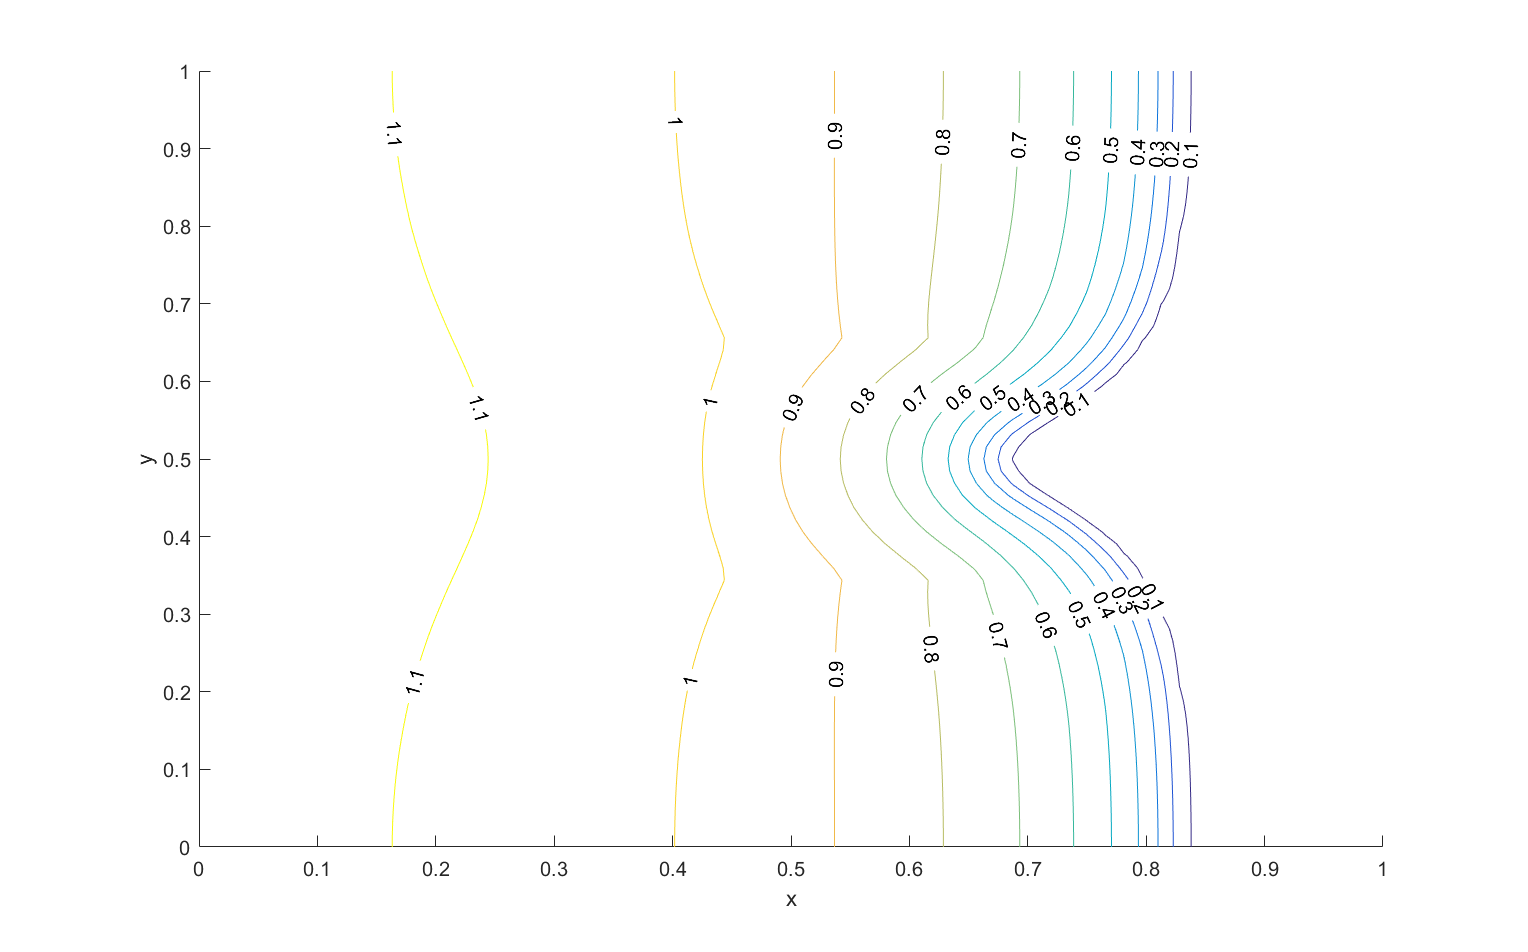
\includegraphics[width=\linewidth]{Example2_1.png}
\caption{Material temperature for Example 2 ($Z=2.5$)}
\label{fig:ex2_1}
\end{figure}

\begin{figure}[htpb!]
\centering
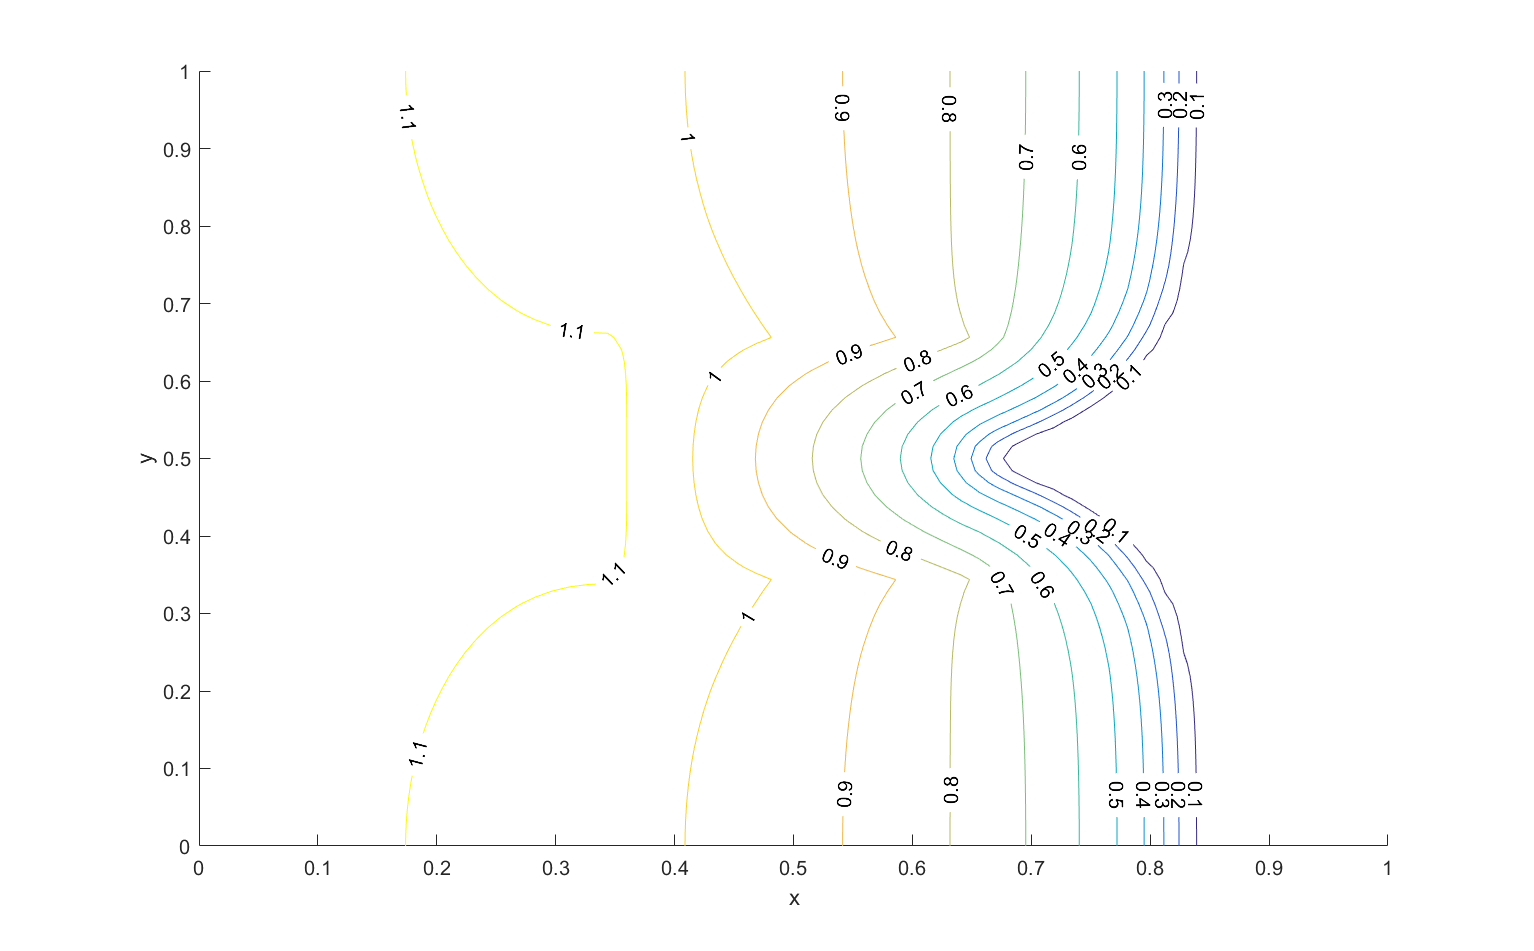
\includegraphics[width=\linewidth]{Example2_2.png}
\caption{Material temperature for Example 2 ($Z=10.0$)}
\label{fig:ex2_2}
\end{figure}


\newpage
%%%%%%%%%%%%%%%%%%%%%%%%%%%%%%%%%%%%%%%%%%%%%%%%%%%%%%%%%%%%%%%%%%%%%%%%%%%%%
%%%%%%%%%%%%%%%%%%%%%%%%%%%%%%%%%%%%%%%%%%%%%%%%%%%%%%%%%%%%%%%%%%%%%%%%%%%%%
\bibliographystyle{abbrvnat}
\bibliography{references}
%%%%%%%%%%%%%%%%%%%%%%%%%%%%%%%%%%%%%%%%%%%%%%%%%%%%%%%%%%%%%%%%%%%%%%%%%%%%%
%%%%%%%%%%%%%%%%%%%%%%%%%%%%%%%%%%%%%%%%%%%%%%%%%%%%%%%%%%%%%%%%%%%%%%%%%%%%%

%%%%%%%%%%%%%%%%%%%%%%%%%%%%%%%%%%%%%%%%%%%%%%%%%%%%%%%%%%%%%%%%%%%%%%%%%%%%%
%%%%%%%%%%%%%%%%%%%%%%%%%%%%%%%%%%%%%%%%%%%%%%%%%%%%%%%%%%%%%%%%%%%%%%%%%%%%%
\end{document}
%%%%%%%%%%%%%%%%%%%%%%%%%%%%%%%%%%%%%%%%%%%%%%%%%%%%%%%%%%%%%%%%%%%%%%%%%%%%%
%%%%%%%%%%%%%%%%%%%%%%%%%%%%%%%%%%%%%%%%%%%%%%%%%%%%%%%%%%%%%%%%%%%%%%%%%%%%%
